
\begin{figure}[H]
  \centering
  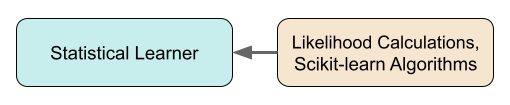
\includegraphics[width=0.7\linewidth]{./chapters/exp2/methodology2_3.png}
  \caption[Third portion of the flowchart from Figure \ref{fig:method2}]
          {Third portion of the flowchart from Figure \ref{fig:method2} being 
           described in this section.}
\end{figure}

The chosen algorithms (\textit{k}-nearest neighbors, decision trees, and
\gls{MLL} calculations) are introduced in Section \ref{sec:algs} and their
implementation details are in Section \ref{sec:statmodel1}.  This section will
therefore only cover the implementation differences from the previous work.
The \gls{MLL} calculations are implemented identically to Chapter
\ref{ch:exp1}.  However, the scikit-learn algorithms in this experiment did
undergo a new round of hyperparameter optimization.

The full list of 22 training sets that undergo training and prediction are as
follows: 
\begin{itemize}
  \item 29 nuclide masses (from Chapter \ref{ch:exp1})
  \item 3 sets of nuclide activities
    \begin{itemize}
      \item 32 nuclide activities (full knowledge scenario for all nuclides, 
            whether or not they are present in a quantity able to be detected)
      \item 12 nuclide activities (full knowledge for long energy windows list)
      \item 7 nuclide activities (full knowledge for short energy windows list)
    \end{itemize}
  \item 18 detector-based processed spectra sets
    \begin{itemize}
      \item Auto energy windows lists applied to six detectors (lab-based 
            \gls{HPGe}, portable \gls{HPGe}, \gls{CZT}, \gls{SrI2}, \gls{LaBr3}, 
            \gls{NaI})
      \item Short energy windows lists applied to six detectors above
      \item Long energy windows lists applied to six detectors above
    \end{itemize}
\end{itemize}

\begin{table}[!htb]
  \centering
  \begin{tabular}{@{}llcll@{}}
    \toprule
    \textbf{\begin{tabular}[c]{@{}l@{}}Training Set\\ Description\end{tabular}} &
    \textbf{\begin{tabular}[c]{@{}l@{}}Prediction\\ Parameter\end{tabular}} &
    \textbf{\begin{tabular}[c]{@{}l@{}}\textit{k} \\ (N neighbors)\end{tabular}} &
    \textbf{\begin{tabular}[c]{@{}l@{}}Max \\ Depth\end{tabular}} &
    \textbf{\begin{tabular}[c]{@{}l@{}}Max \\ Features\end{tabular}} \\ 
    \toprule
    \multirow{4}{*}{\begin{tabular}[c]
    {@{}l@{}}29 \\ Nuclide\\ Masses\end{tabular}}          & Reactor Type & 4 & 56 & 29          \\
                                                           & Burnup       & 1 & 77 & 29          \\
                                                           & Enrichment   & 1 & 73 & 29          \\
                                                           & Cooling Time & 2 & 45 & 29          \\ 
                                                           \hline
    \multirow{4}{*}{\begin{tabular}[c]
    {@{}l@{}}32\\ Nuclide\\ Activities\end{tabular}}       & Reactor Type & 1 & 41 & 32          \\
                                                           & Burnup       & 1 & 49 & 32          \\
                                                           & Enrichment   & 1 & 67 & 32          \\
                                                           & Cooling Time & 7 & 56 & 32          \\
                                                           \hline
    \multirow{4}{*}{\begin{tabular}[c]
    {@{}l@{}}7 or 12\\ Nuclide \\ Activities\end{tabular}} & Reactor Type & 1 & 67 & 7 or 12     \\
                                                           & Burnup       & 1 & 78 & 7 or 12     \\
                                                           & Enrichment   & 1 & 60 & 7 or 12     \\
                                                           & Cooling Time & 4 & 68 & 7 or 12     \\
                                                           \hline
    \multirow{4}{*}{\begin{tabular}[c]
    {@{}l@{}}Energy \\ Windows:\\ Short\end{tabular}}      & Reactor Type & 1 & 62 & 42          \\
                                                           & Burnup       & 1 & 62 & 42          \\
                                                           & Enrichment   & 4 & 64 & 42          \\
                                                           & Cooling Time & 2 & 54 & 42          \\
                                                           \hline
    \multirow{4}{*}{\begin{tabular}[c]
    {@{}l@{}}Energy \\ Windows:\\ Long\end{tabular}}       & Reactor Type & 4 & 62 & 151         \\
                                                           & Burnup       & 1 & 51 & 151         \\
                                                           & Enrichment   & 5 & 73 & 151         \\
                                                           & Cooling Time & 2 & 64 & 151         \\
                                                           \hline
    \multirow{4}{*}{\begin{tabular}[c]
    {@{}l@{}}Energy \\ Windows:\\ Auto\end{tabular}}       & Reactor Type & 2 & 61 & None or 150 \\
                                                           & Burnup       & 1 & 52 & None or 150 \\
                                                           & Enrichment   & 4 & 67 & None or 150 \\
                                                           & Cooling Time & 2 & 58 & None or 150 \\ 
    \bottomrule 
  \end{tabular}
  \caption[Optimized algorithm hyperparameters for all training sets in second 
           experiment]
          {Optimized algorithm hyperparameters; the energy lists took all 
           detectors into account.}
  \label{tbl:exp2hypparam}
\end{table}

Table \ref{tbl:exp2hypparam} lists the hyperparameter optimization results for
the 22 training sets. Because the 29 nuclide mass training set is included in
this chapter for comparison, its optimization results are also listed here.
The number of features for decision trees are not limited because the test runs
for optimization provided highly variable results. The only case where this is
not true is with the auto energy windows list for the lab-based \gls{HPGe} with
a length of 206; the maximum features for this one case are limited to 150.
Instead, optimization was carried out only on the maximum depth for decision
trees with keeping the full length of features.  This is an area that could
undergo deeper exploration than what occurs in this work, since the training
sets with large feature sets can become overfit.

The optimization took place in two rounds, where the first round had a coarser
grid of \textit{k} for \textit{k}-nearest neighbors and maximum depth for
decision trees and the second round had a finer grid of parameters. The 7 \& 12
nuclide activity training sets were optimized separately but contain averages
of the two results for the maximum depth, and the higher value of \textit{k}
when the two did not match. The \textit{k} and maximum depths were averaged
across all six detectors for each energy window list length (short, long, and
auto).  There were fairly consistent results from the short and long lists, but
the variable length of the auto-generated energy windows lists (in Table
\ref{tbl:enwindows}) gave a wider range of ideal hyperparameters.

